\section{Validation of the analysis package}
\label{sec:validation}

In this section the validation of the MLHEP package, which is performed with respect to the standard AliPhysics Analysis Tasks for the \Ds meson and the \Lc baryon, is presented. This section validates the calculations performed in the package itself, but this depends obviously on the correct filling of the input TTrees. Therefore, when new analyses will start to use the framework, still some validation checks should be perfomed on the TTree creators.

As described above, the relevant output of the MLHEP package are root files containing the extracted raw yields, prompt and feed-down efficiencies, and the normalised number of events. These three calculations will be validated with the standard tasks (AliAnalysisTaskSEDs for \Ds and AliAnalysisTaskSELc2V0bachelor + AliCFVertexingHFLctoV0bachelor for \Lc) in the subsections below.

\subsection{Candidate selection and invariant distributions}
\label{subsec:invMassValidation}

In Fig.~\ref{fig:InvMassDsComparisonMCpp} and \ref{fig:InvMassLcComparisonMCDataPbPb} the comparison at invariant mass level is shown for \Ds and \Lc respectively. Both the standard analysis bit, and the custom cut selection were enabled in the MLHEP package, and compared to the output of the standard tasks.

\begin{figure}[b!]
\begin{center}
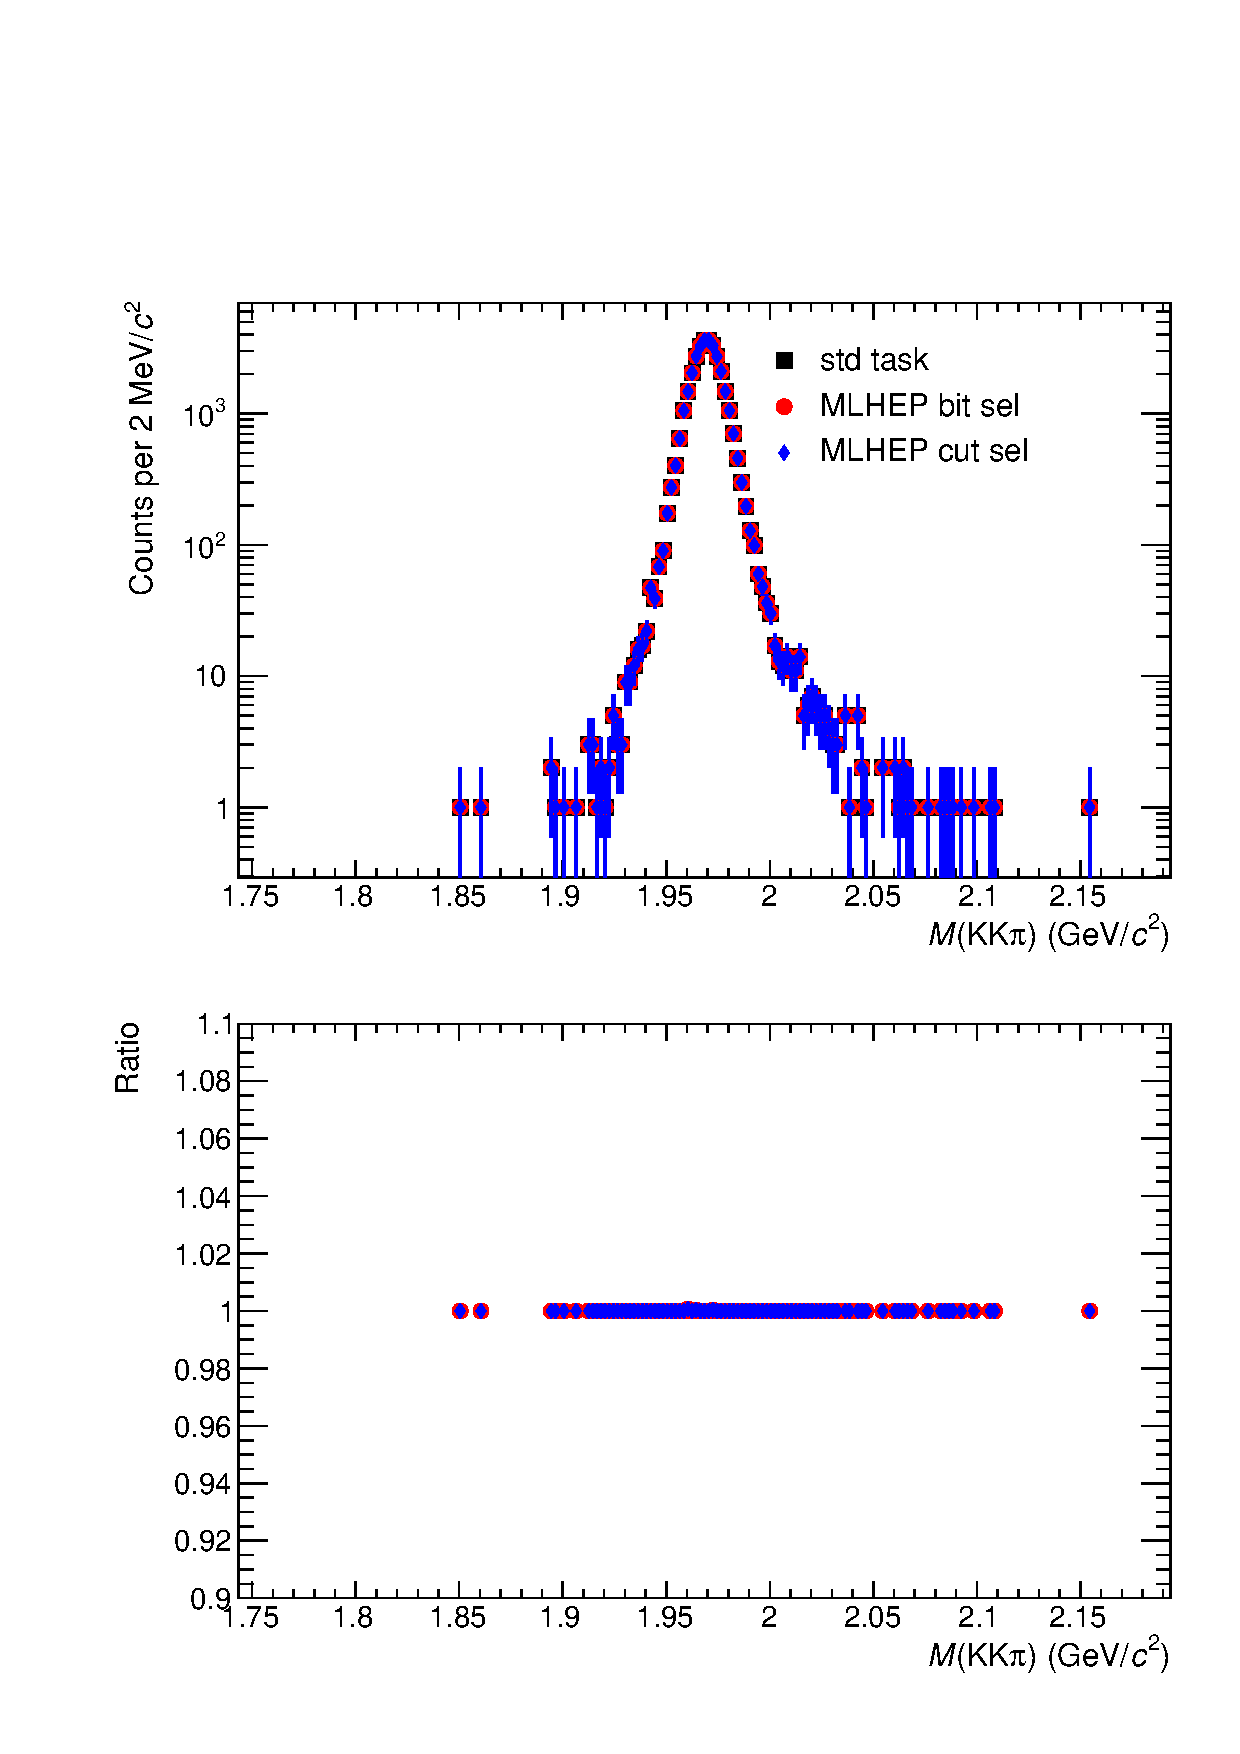
\includegraphics[width=0.45\textwidth]{figures/DsInvMassComparison.pdf}
\caption{Invariant-mass distribution of signal (prompt and feed-down) $\Ds$ candidates with $2<\pt<24~\GeV/c$ obtained from the LHC18a4a2 MC production for pp collisions at $\sqrt{s}=5.02~\TeV$ with the AliAnalysisTaskDs task and the MachineLearningHEP package. The same selections used in~\cite{Acharya:2019mgn} were applied. The ratio of the different distributions is shown in the bottom plot.}
\label{fig:InvMassDsComparisonMCpp}
\end{center}
\end{figure}

\begin{figure}[tb!]
\begin{center}
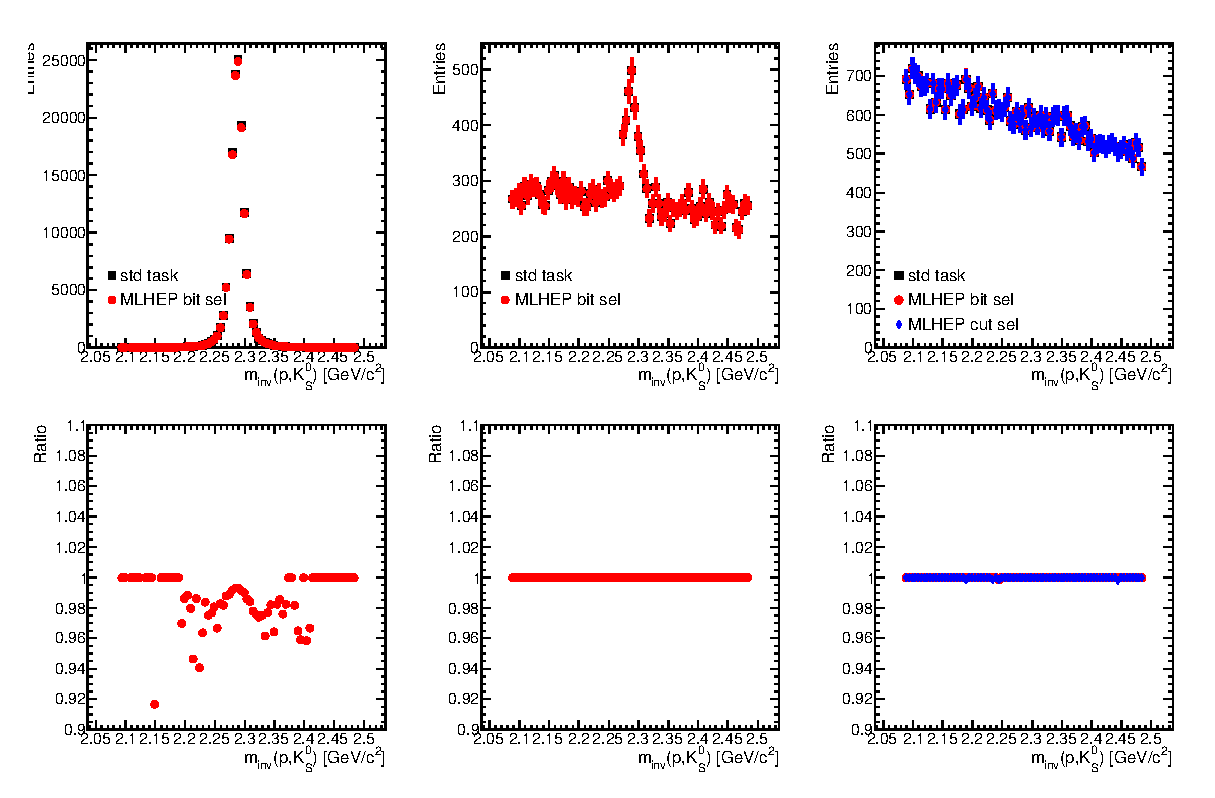
\includegraphics[width=0.9\textwidth]{figures/LcInvMassComparison.eps}
\caption{Left: Invariant-mass distributions of signal (prompt and feed-down) $\Lc$ candidates from the LHC19c2b MC production for Pb-Pb collisions at $\sqrt{s}=5.02~\TeV$. Middle: Invariant-mass distributions of all $\Lc$ candidates from the LHC19c2b MC production ran as it was data. Right: Invariant-mass distributions of all $\Lc$ candidates from the LHC18r PbPb production. All spectra are transverse momentum integrated, and obtained with the AliAnalysisTaskSELc2V0bachelor task and the MachineLearningHEP package. The ratio of the different distributions is shown in the bottom plots.}
\label{fig:InvMassLcComparisonMCDataPbPb}
\end{center}
\end{figure}

For the $\Ds$ meson an almost 100\% match is observed. The very few entries that differ are understood: It is coming from rounding in the pandas dataframe and a very small bug in the standard $\Ds$ task that only affected MC (has been fixed in the meantime). The same is observed for the $\Lc$ baryon for data and MC ran as it was data. Here, the very few entries that differ are only due to rounding in the dataframes. For MC a difference of a few percent is observed, but also this difference is understood. It is due to different ways of tagging what is signal (e.g. ${\rm X}_{\rm not \, c/b} \rightarrow {\rm B} + {\rm X}_{1} \rightarrow \Lc + {\rm X}_{2}$, which is considered as signal in the standard task, but background in the MLHEP package). When the same conventions are used, a perfect match is obtained, similar as for data. \textcolor{red}{[Plot to be produced?]}

\subsection{Efficiency}
\label{subsec:effValidation}

In Fig.~\ref{fig:EffDsComparisonMCpp} and \ref{fig:EffLcComparisonMCPbPb} the comparison at efficiency level for both prompt and feed-down is shown for \Ds and \Lc respectively. Both the standard analysis bit, and the custom cut selection were enabled in the MLHEP package, and compared to the output of the standard \Ds task and the CorrectionFramework or the \Lc.
- Comparison efficiency from the package and RecoPID/GenLimAcc from correction framework

\begin{figure}[tb]
\begin{center}
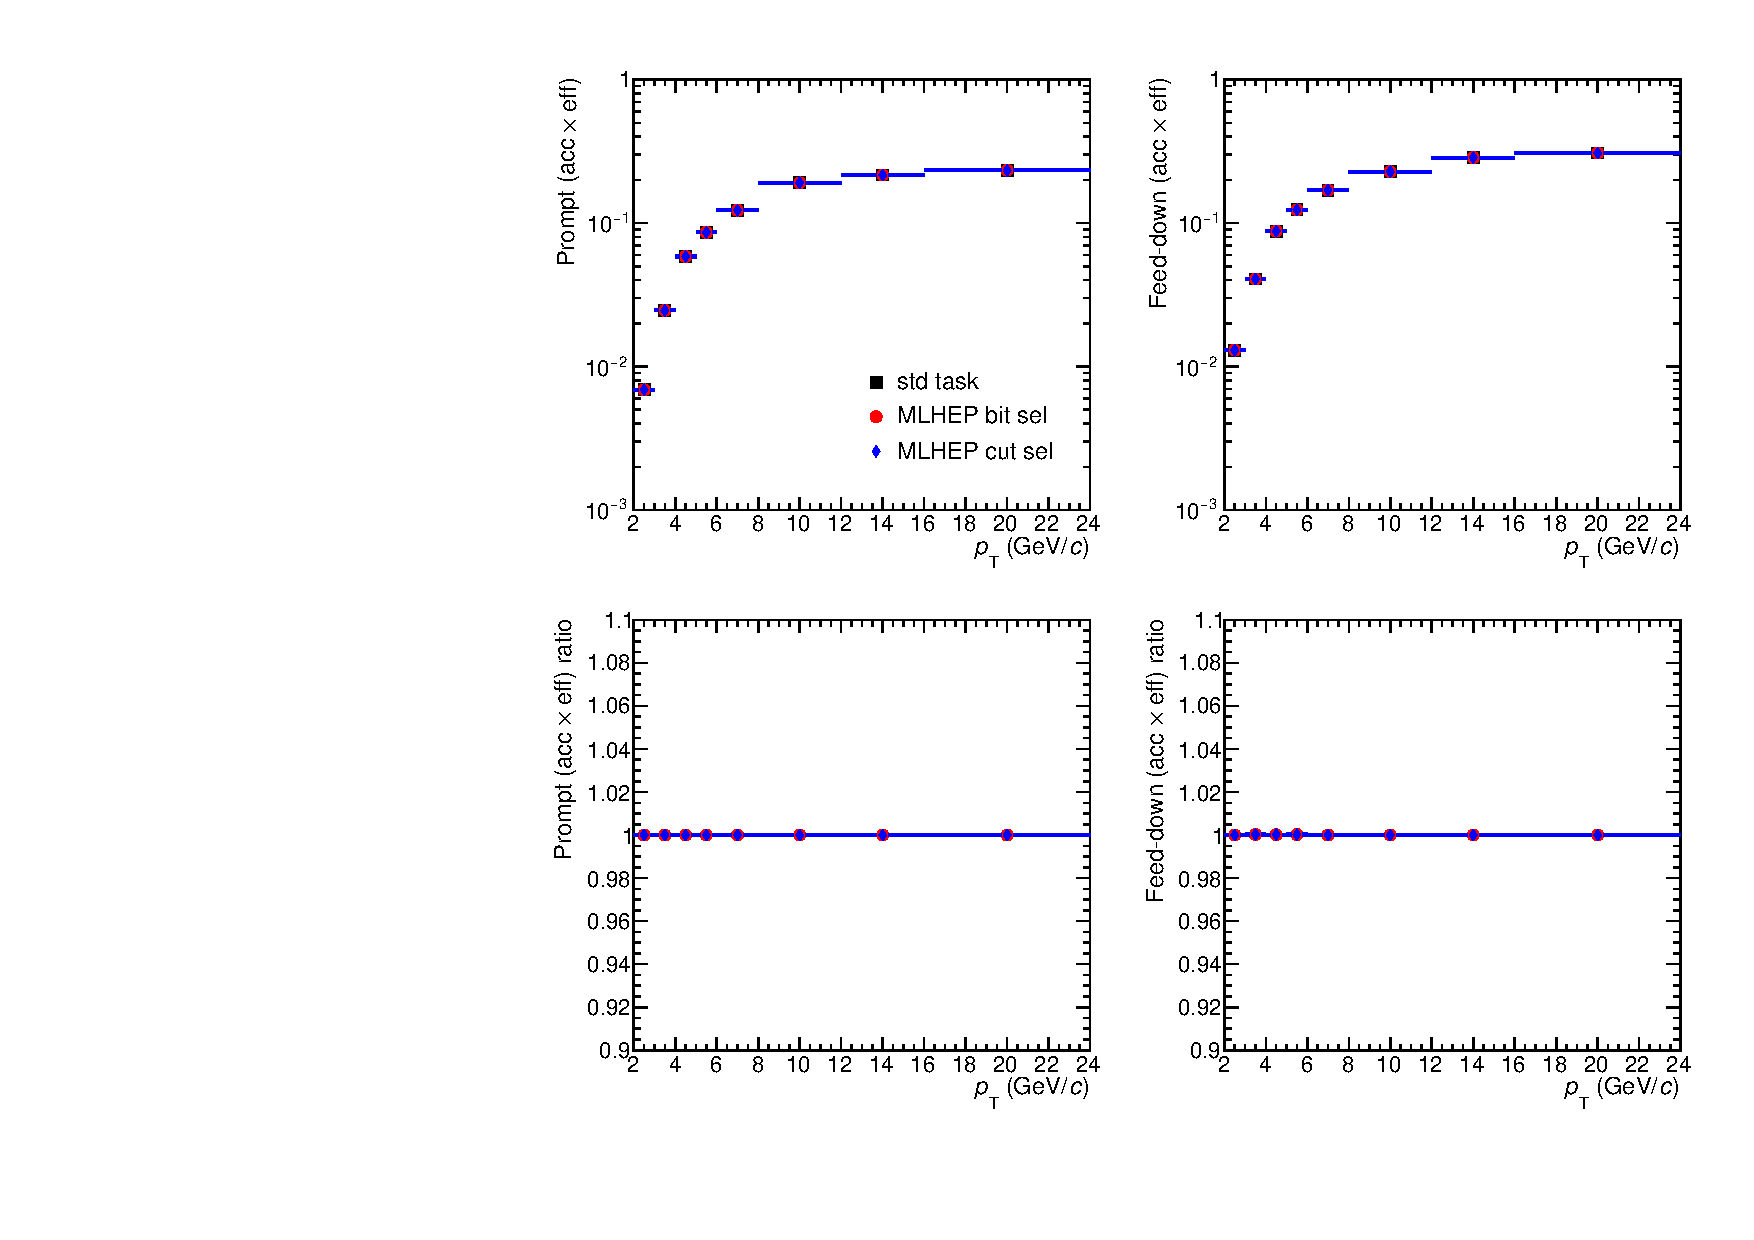
\includegraphics[width=0.7\textwidth]{figures/DsEfficiencyComparison.pdf}
\caption{Acceptance times efficiency factors of prompt (left) and feed-down (right) $\Ds$ for different \pt bins obtained from the LHC18a4a2 MC production for pp collisions at $\sqrt{s}=5.02~\TeV$ with the AliAnalysisTaskDs task and the MachineLearningHEP package. The same selections used in~\cite{Acharya:2019mgn} were applied. The ratio of the different distributions is shown in the bottom plots.}
\label{fig:EffDsComparisonMCpp} 
\end{center}
\end{figure}

\begin{figure}[tb]
\begin{center}
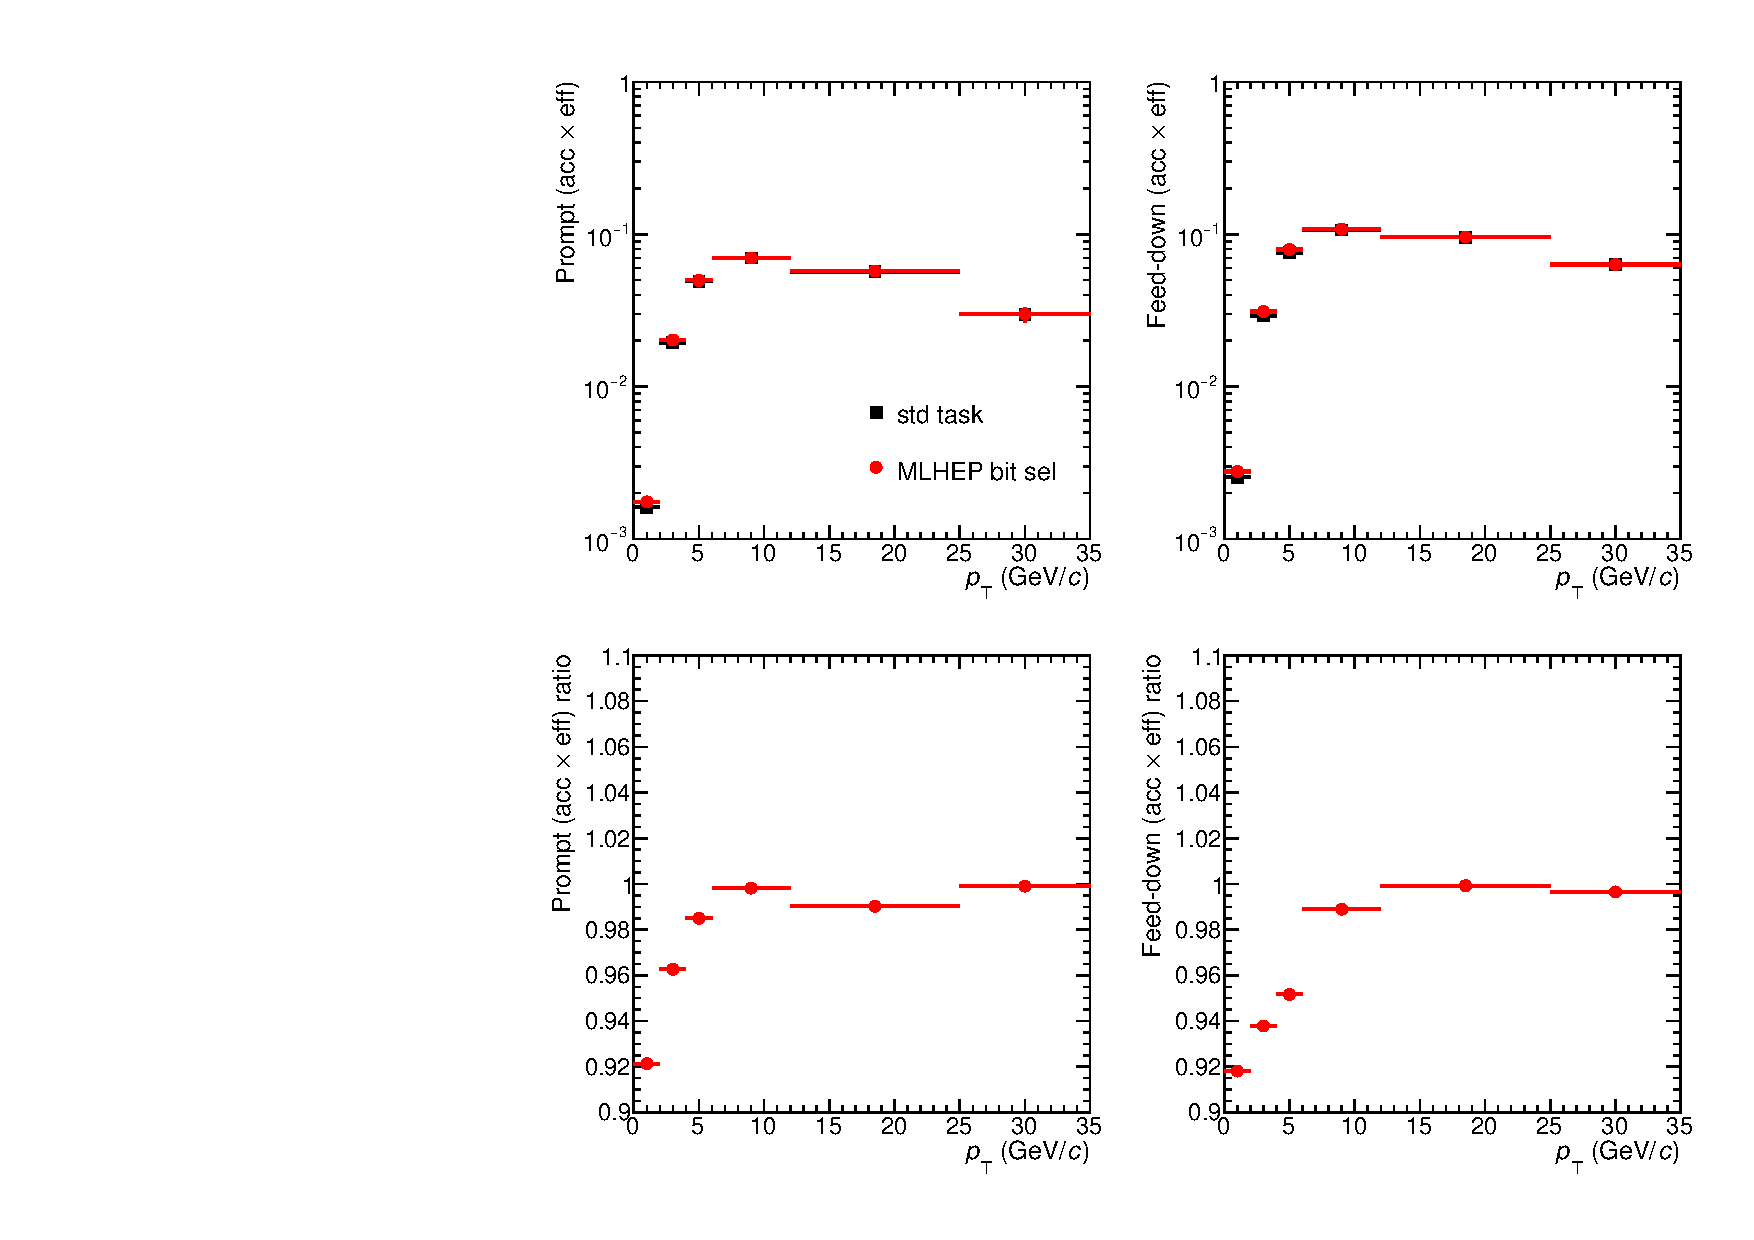
\includegraphics[width=0.7\textwidth]{figures/LcEfficiencyComparison.pdf}
\caption{Acceptance times efficiency factors of prompt (left) and feed-down (right) $\Lc$ for different \pt bins obtained from the LHC19c3b MC production for PbPb collisions at $\sqrt{s}=5.02~\TeV$ with the AliCFVertexingHFLctoV0bachelor task and the MachineLearningHEP package. The ratio of the different distributions is shown in the bottom plots. }
\label{fig:EffLcComparisonMCPbPb}
\end{center}
\end{figure}

\subsection{Normalisation}
\label{subsec:normValidation}

The number of events used to compute the integrated luminosity, which enters in the calculation of the cross section, calculated by the new framework is compared to the number obtained from AliNormalizationCounter (PWGHF/vertexingHF/AliNormalizationCounter.h), see Fig.~\ref{fig:NormalisationComparisonMCpp}. The number of events selected by AliRDHFCuts::IsEventSelected is corrected to take into account the events for which the primary vertex is not reconstructed and $|z_{vtx}|<10$~cm. A perfect agreement is observed when comparing the MachineLearningHEP package with the standard tool for both the \Ds and \Lc.
 
 \begin{figure}[tb]
\begin{center}
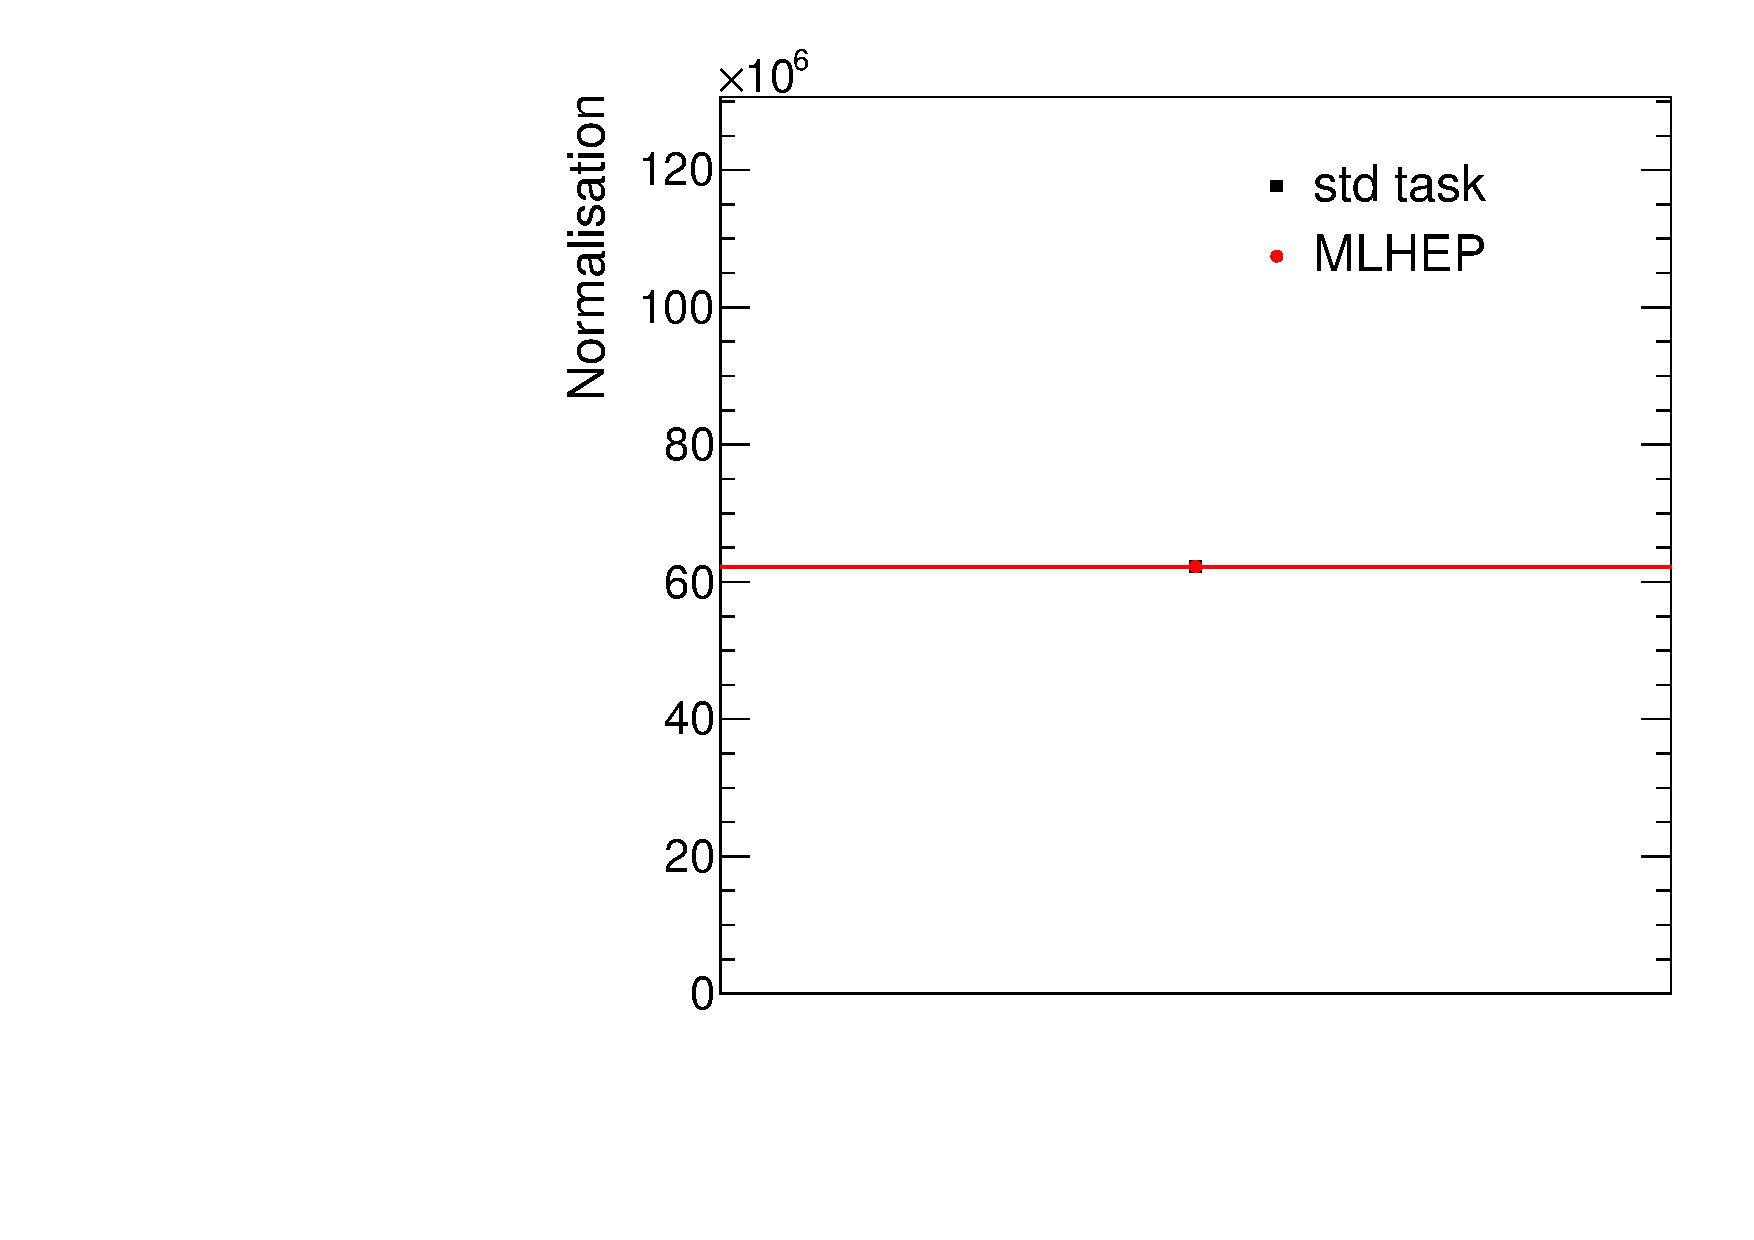
\includegraphics[width=0.35\textwidth]{figures/NormComparison.pdf}
\caption{Comparison of the normalisation factor obtained from the LHC18a4a2 MC production for pp collisions at $\sqrt{s}=5.02~\TeV$ with the AliNormalizationCounter and the MachineLearningHEP package.}
\label{fig:NormalisationComparisonMCpp} 
\end{center}
\end{figure}
